% Architecture of the Lean-in-the-loop RL system (standalone figure).
% Build: latexmk -pdf -interaction=nonstopmode lean_loop_architecture.tex
\documentclass[border=6pt]{standalone}
\usepackage[T1]{fontenc}
\usepackage{lmodern}
\usepackage{amsmath,amssymb}
\usepackage{xcolor}
\usepackage{tikz}
\usetikzlibrary{arrows.meta,positioning,shapes.geometric,calc,fit,decorations.pathreplacing,backgrounds}

% Shared diagram styles, copied from docs/tex/project_report.tex.
\tikzset{
  box/.style={draw, rounded corners, align=center, font=\small, minimum height=0.8cm, inner sep=4pt},
  good/.style={box, fill=green!15},
  bad/.style={box, fill=red!10},
  plain/.style={box, fill=gray!8},
  arr/.style={-{Latex[length=2.2mm]}, thick},
  fail/.style={-{Latex[length=2.2mm]}, dashed, red!60!black},
  note/.style={font=\footnotesize, align=center},
}
% Figure-local styles.
\tikzset{
  frame/.style={draw, rounded corners, thick, inner sep=6pt},
  part/.style={box, font=\footnotesize, text width=#1, align=flush center},
  part/.default=4.5cm,
  tok/.style={draw, fill=white, font=\footnotesize, minimum width=0.7cm, minimum height=0.55cm},
  ttl/.style={font=\small\bfseries, anchor=west},
  tag/.style={font=\small\bfseries},
}

\begin{document}
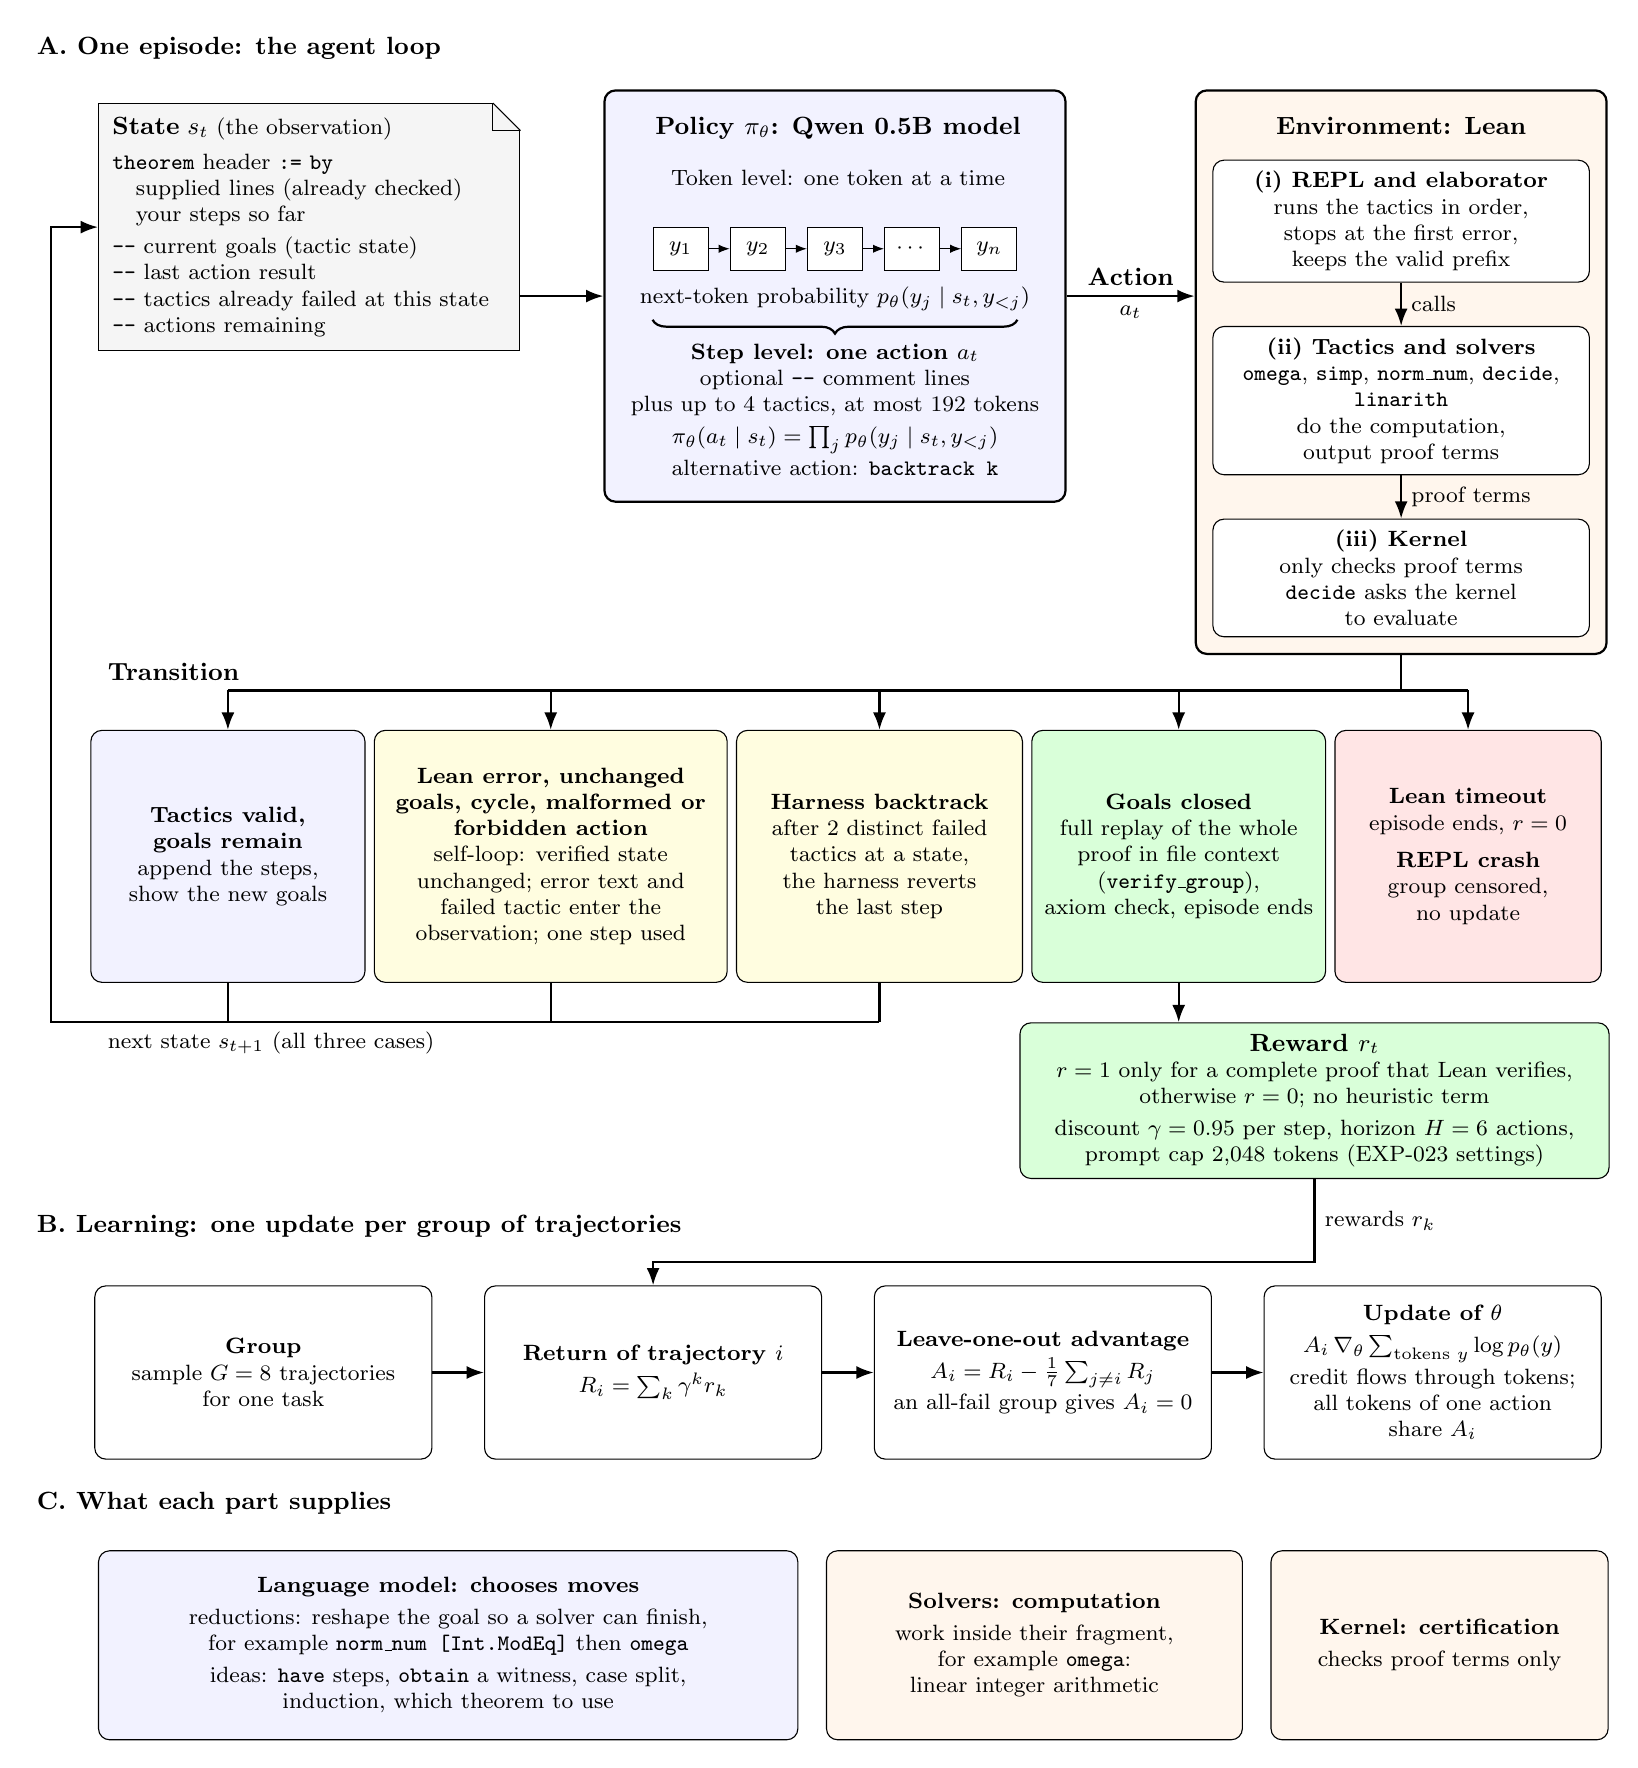
\begin{tikzpicture}

% ------------------------------------------------------------------
% A. One episode
% ------------------------------------------------------------------
\node[ttl] at (-0.9, 1.1) {A. One episode: the agent loop};

% State s_t, drawn as a small Lean file.
\node[draw, fill=gray!8, text width=5.0cm, align=left, font=\footnotesize,
      inner sep=5pt, anchor=north west] (state) at (0, 0.4) {%
  \textbf{\small State $s_t$} (the observation)\\[3pt]
  \texttt{theorem} header \texttt{:= by}\\
  \quad supplied lines (already checked)\\
  \quad your steps so far\\[2pt]
  \texttt{-{}-} current goals (tactic state)\\
  \texttt{-{}-} last action result\\
  \texttt{-{}-} tactics already failed at this state\\
  \texttt{-{}-} actions remaining};
\fill[white] ($(state.north east)+(-0.35,0)$) -- (state.north east) -- ($(state.north east)+(0,-0.35)$) -- cycle;
\draw ($(state.north east)+(-0.35,0)$) -- ($(state.north east)+(-0.35,-0.35)$) -- ($(state.north east)+(0,-0.35)$);
\draw ($(state.north east)+(-0.35,0)$) -- ($(state.north east)+(0,-0.35)$);

% Policy: the language model, with token level and step level.
\node[font=\small\bfseries, anchor=north] (pt) at (9.4, 0.35) {Policy $\pi_\theta$: Qwen 0.5B model};
\node[note, below=0.15cm of pt] (tl) {Token level: one token at a time};
\foreach \i/\s in {1/$y_1$, 2/$y_2$, 3/$y_3$, 4/$\cdots$, 5/$y_n$}
  \node[tok] (k\i) at (7.4+0.98*\i-0.98, -1.45) {\s};
\foreach \a/\b in {1/2, 2/3, 3/4, 4/5} \draw[-{Latex[length=1.4mm]}] (k\a) -- (k\b);
\node[note, below=0.08cm of k3] (np) {next-token probability $p_\theta(y_j \mid s_t, y_{<j})$};
\draw[decorate, decoration={brace, mirror, amplitude=5pt}, thick]
  ($(k1.south west)+(0,-0.62)$) -- ($(k5.south east)+(0,-0.62)$) coordinate[midway] (bmid);
\node[note, below=0.18cm of bmid] (sl) {%
  \textbf{Step level: one action $a_t$}\\
  optional \texttt{-{}-} comment lines\\
  plus up to 4 tactics, at most 192 tokens\\[2pt]
  $\pi_\theta(a_t \mid s_t) = \prod_j p_\theta(y_j \mid s_t, y_{<j})$\\[2pt]
  alternative action: \texttt{backtrack k}};
\begin{scope}[on background layer]
  \node[frame, fill=blue!5, fit=(pt)(tl)(k1)(k5)(np)(sl)] (pol) {};
\end{scope}

% Lean: elaborator, solvers, kernel.
\node[font=\small\bfseries, anchor=north] (lt) at (16.55, 0.35) {Environment: Lean};
\node[part, fill=white, below=0.2cm of lt] (repl) {%
  \textbf{(i) REPL and elaborator}\\
  runs the tactics in order,\\
  stops at the first error,\\
  keeps the valid prefix};
\node[part, fill=white, below=0.55cm of repl] (solv) {%
  \textbf{(ii) Tactics and solvers}\\
  \texttt{omega}, \texttt{simp}, \texttt{norm\_num}, \texttt{decide}, \texttt{linarith}\\
  do the computation,\\
  output proof terms};
\node[part, fill=white, below=0.55cm of solv] (kern) {%
  \textbf{(iii) Kernel}\\
  only checks proof terms\\
  \texttt{decide} asks the kernel\\ to evaluate};
\draw[arr] (repl) -- node[right, note] {calls} (solv);
\draw[arr] (solv) -- node[right, note] {proof terms} (kern);
\begin{scope}[on background layer]
  \node[frame, fill=orange!7, fit=(lt)(repl)(solv)(kern)] (lean) {};
\end{scope}

% Loop arrows: state to policy to Lean.
\draw[arr] (state.east |- pol.west) -- (pol.west);
\draw[arr] (pol.east) -- node[above, tag] {Action} node[below, note] {$a_t$} (pol.east -| lean.west);

% Transition bus from Lean to five outcome boxes.
\coordinate (tb) at ($(lean.south)+(0,-0.95)$);
\begin{scope}[every node/.style={part=3.45cm, minimum height=3.2cm, anchor=north}]
  \node[fill=blue!5, text width=3.2cm]  (t1) at (1.65,0 |- tb) {%
    \textbf{Tactics valid,}\\ \textbf{goals remain}\\
    append the steps,\\ show the new goals};
  \node[fill=yellow!12, text width=4.2cm] (t2) at (5.75,0 |- tb) {%
    \textbf{Lean error, unchanged}\\ \textbf{goals, cycle, malformed or}\\ \textbf{forbidden action}\\
    self-loop: verified state\\ unchanged; error text and\\ failed tactic enter the\\ observation; one step used};
  \node[fill=yellow!12, text width=3.35cm] (t3) at (9.925,0 |- tb) {%
    \textbf{Harness backtrack}\\
    after 2 distinct failed\\ tactics at a state,\\ the harness reverts\\ the last step};
  \node[fill=green!15, text width=3.45cm] (t4) at (13.725,0 |- tb) {%
    \textbf{Goals closed}\\
    full replay of the whole\\ proof in file context\\ (\texttt{verify\_group}),\\ axiom check, episode ends};
  \node[fill=red!10, text width=3.1cm] (t5) at (17.4,0 |- tb) {%
    \textbf{Lean timeout}\\ episode ends, $r = 0$\\[4pt]
    \textbf{REPL crash}\\ group censored,\\ no update};
\end{scope}
\coordinate (bus) at ($(lean.south)+(0,-0.45)$);
\draw[thick] (lean.south) -- (bus);
\draw[thick] (t1.north |- bus) -- (t5.north |- bus);
\foreach \t in {t1,t2,t3,t4,t5} \draw[arr] (\t.north |- bus) -- (\t.north);
\node[tag, anchor=south west] at (0.0,0 |- bus) {Transition};

% Return path to the next state.
\coordinate (rb) at ($(t1.south)+(0,-0.5)$);
\coordinate (ret) at (-0.6,0 |- rb);
\foreach \t in {t1,t2,t3} \draw[thick] (\t.south) -- (\t.south |- ret);
\draw[arr] (t3.south |- ret) -- (ret) |- (state.west);
\node[note, anchor=north west] at (0.0,0 |- rb) {next state $s_{t+1}$ (all three cases)};

% Reward.
\node[good, font=\footnotesize, text width=7.2cm, align=flush center, anchor=north] (rew) at ($(t4.south -| 15.45,0)+(0,-0.5)$) {%
  \textbf{\small Reward $r_t$}\\
  $r = 1$ only for a complete proof that Lean verifies,\\
  otherwise $r = 0$; no heuristic term\\[2pt]
  discount $\gamma = 0.95$ per step, horizon $H = 6$ actions,\\
  prompt cap 2,048 tokens (EXP-023 settings)};
\draw[arr] (t4.south) -- (t4.south |- rew.north);

% ------------------------------------------------------------------
% B. Learning
% ------------------------------------------------------------------
\coordinate (lb) at ($(rew.south)+(0,-1.35)$);
\node[ttl] (bt) at ($(-0.9,0 |- lb)+(0,0.75)$) {B. Learning: one update per group of trajectories};
\begin{scope}[every node/.style={part=4.0cm, minimum height=2.2cm, anchor=north, fill=white}]
  \node (l1) at (2.1,0 |- lb) {%
    \textbf{Group}\\ sample $G = 8$ trajectories\\ for one task};
  \node (l2) at (7.05,0 |- lb) {%
    \textbf{Return of trajectory $i$}\\[2pt] $R_i = \sum_k \gamma^k r_k$};
  \node (l3) at (12.0,0 |- lb) {%
    \textbf{Leave-one-out advantage}\\[2pt]
    $A_i = R_i - \frac{1}{7}\sum_{j \neq i} R_j$\\[2pt]
    an all-fail group gives $A_i = 0$};
  \node (l4) at (16.95,0 |- lb) {%
    \textbf{Update of $\theta$}\\[2pt]
    $A_i \, \nabla_\theta \sum_{\text{tokens } y} \log p_\theta(y)$\\[2pt]
    credit flows through tokens;\\ all tokens of one action\\ share $A_i$};
\end{scope}
\foreach \a/\b in {l1/l2, l2/l3, l3/l4} \draw[arr] (\a) -- (\b);
\draw[arr] (rew.south) -- node[right, note] {rewards $r_k$} ($(rew.south |- lb)+(0,0.3)$) -| (l2.north);

% ------------------------------------------------------------------
% C. Legend
% ------------------------------------------------------------------
\coordinate (cb) at ($(l4.south)+(0,-1.15)$);
\node[ttl] at ($(-0.9,0 |- cb)+(0,0.6)$) {C. What each part supplies};
\begin{scope}[every node/.style={part, minimum height=2.4cm, anchor=north west}]
  \node[part=8.6cm, minimum height=2.4cm, fill=blue!5] (c1) at (0,0 |- cb) {%
    \textbf{Language model: chooses moves}\\[2pt]
    reductions: reshape the goal so a solver can finish,\\
    for example \texttt{norm\_num [Int.ModEq]} then \texttt{omega}\\[2pt]
    ideas: \texttt{have} steps, \texttt{obtain} a witness, case split,\\
    induction, which theorem to use};
  \node[part=5.0cm, minimum height=2.4cm, fill=orange!7] (c2) at ($(c1.north east)+(0.35,0)$) {%
    \textbf{Solvers: computation}\\[2pt]
    work inside their fragment,\\
    for example \texttt{omega}:\\ linear integer arithmetic};
  \node[part=4.0cm, minimum height=2.4cm, fill=orange!7] (c3) at ($(c2.north east)+(0.35,0)$) {%
    \textbf{Kernel: certification}\\[2pt]
    checks proof terms only};
\end{scope}

\end{tikzpicture}
\end{document}
